\documentclass[12pt]{article}

\usepackage{amsmath, color}
\usepackage{mdwmath}
\usepackage{amssymb, epsf, epsfig, textcomp}
\renewcommand{\baselinestretch}{1.3}
\usepackage{a4wide}
\newcommand{\argmin}{\mathop{\mathrm{argmin}}}
\usepackage{caption}
\usepackage{subcaption}
\usepackage{mathtools}
\usepackage{listings}
\lstdefinestyle{myCustomMatlabStyle}{
	basicstyle=\ttfamily\footnotesize,
	breaklines=true,
	language=Matlab,
	numbers=left,
	stepnumber=1,
	numbersep=10pt,
	tabsize=4,
	showspaces=false,
	showstringspaces=false
}
\begin{document}
	\noindent\rule{\textwidth}{2pt}
	\begin{center}
		{\bf Technical University of Crete}\\
		{\bf School of Electrical and Computer Engineering} \\
		Course: {\bf Reinforcement Learning and Dynamic Optimization} \\
		Assignment 1 \\%(120/1000) \\
		Report Delivery Date: Sunday, March 26, 2023 \\
	\end{center}
	{\bf Student: }Alevrakis Dimitrios 2017030001\\
	\rule{\textwidth}{.5pt}
	\vskip .1cm
	\noindent\\
	
		\begin{enumerate}
			\item
			\begin{figure}[h!]
				\centering
				\begin{subfigure}[b]{0.3\textwidth}
					\centering
					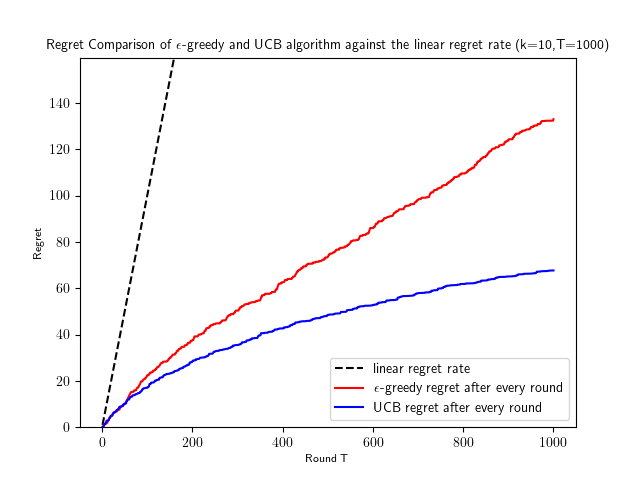
\includegraphics[width=\textwidth]{fig0.png}
					\caption{$(k=10, T=1000)$}
				\end{subfigure}
				\hfill
				\begin{subfigure}[b]{0.3\textwidth}
					\centering
					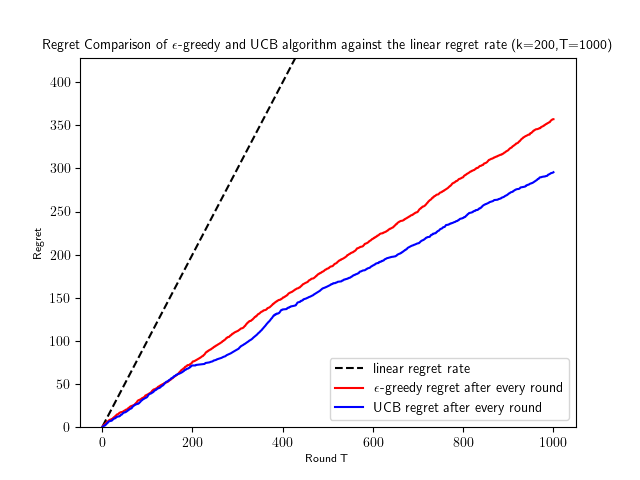
\includegraphics[width=\textwidth]{fig1.png}
					\caption{$(k=200, T=1000)$}
				\end{subfigure}
				
				\begin{subfigure}[b]{0.3\textwidth}
					\centering
					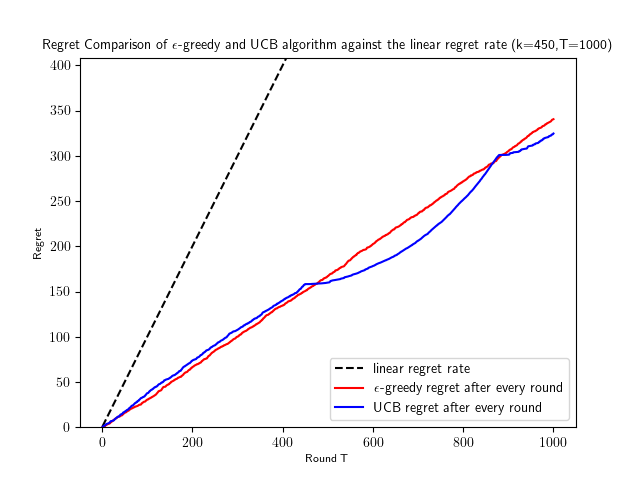
\includegraphics[width=\textwidth]{fig3.png}
					\caption{$(k=450, T=1000)$}
				\end{subfigure}
				\hfill
				\begin{subfigure}[b]{0.3\textwidth}
					\centering
					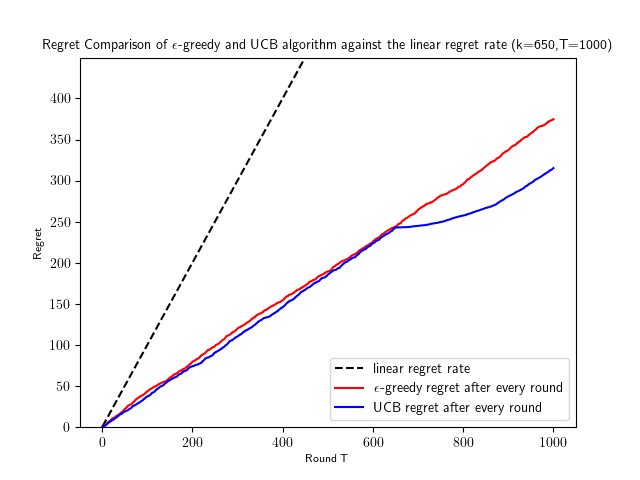
\includegraphics[width=\textwidth]{fig4.png}
					\caption{$(k=650, T=1000)$}
				\end{subfigure}
				\hfill
				\begin{subfigure}[b]{0.3\textwidth}
					\centering
					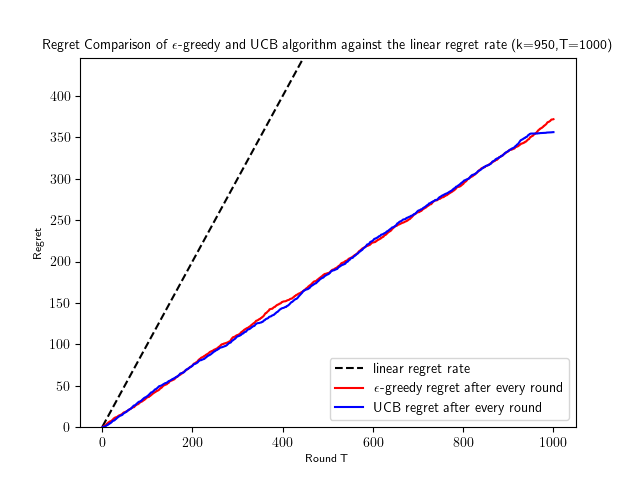
\includegraphics[width=\textwidth]{fig9.png}
					\caption{$(k=950, T=1000)$}
				\end{subfigure}
				\caption{$(k\in[10,950], T=1000)$}			
			\end{figure}
			
			
			In the experiments of figure 1, we are testing the effect that the ratio $\frac{k}{T}$ has on the performance of both algorithms.\\
			We can observe that, when $k\ll T$ the UCB algorithms achieves a distinguishably lesser regret rate and thus lower regret at the horizon.\\
			Though, when $k<\frac{1}{2}T$ the UCB algorithm has slightly lower regret rate and achieves a lower regret at the horizon but by a significantly lesser margin.\\
			When $k$ can be considered $k\approxeq \frac{1}{2}T$ the algorithms have similar regret rates. Worth noting that UCB presents "spikes" where the regret becomes lower than t $\epsilon$-greedy but after again equalizing as shown in figure 1 (c) and (d). Those spikes are probably due to the algorithm choosing the best hand but afterwards switching.\\
			Lastly when $k\approx T$ both algorithms present the same regret rate. \\
			
			\begin{figure}[h!]
				\centering
				\begin{subfigure}[b]{0.3\textwidth}
					\centering
					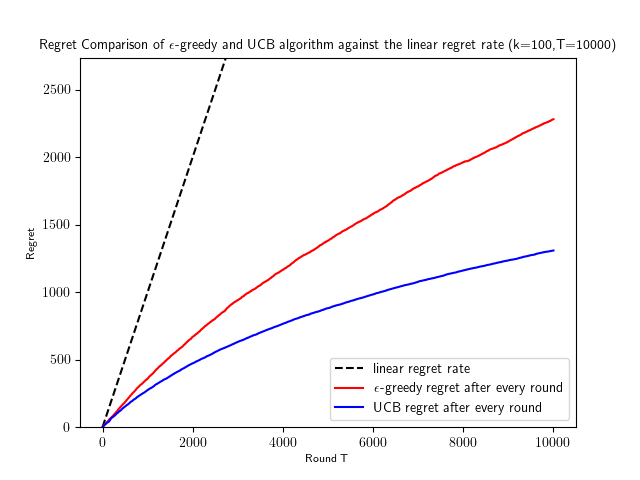
\includegraphics[width=\textwidth]{fig5.png}
					\caption{$(k=100, T=10000)$}
				\end{subfigure}
				\hfill
				\begin{subfigure}[b]{0.3\textwidth}
					\centering
					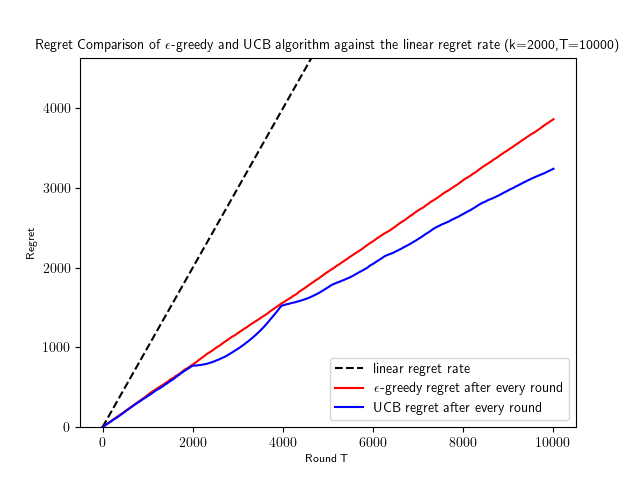
\includegraphics[width=\textwidth]{fig6.png}
					\caption{$(k=2000, T=10000)$}
				\end{subfigure}
				
				\begin{subfigure}[b]{0.3\textwidth}
					\centering
					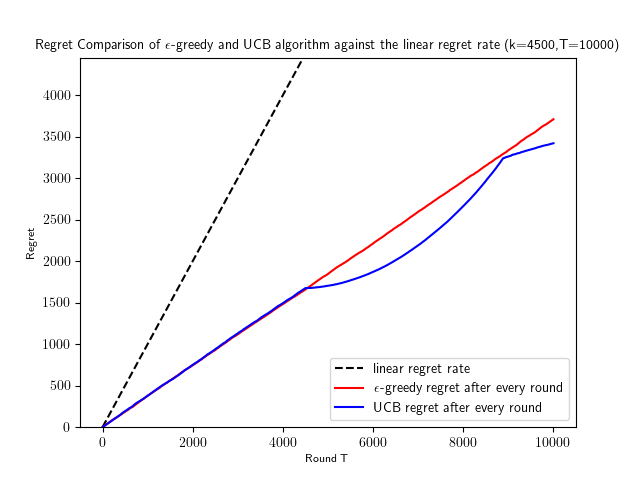
\includegraphics[width=\textwidth]{fig7.png}
					\caption{$(k=4500, T=10000)$}
				\end{subfigure}
				\hfill
				\begin{subfigure}[b]{0.3\textwidth}
					\centering
					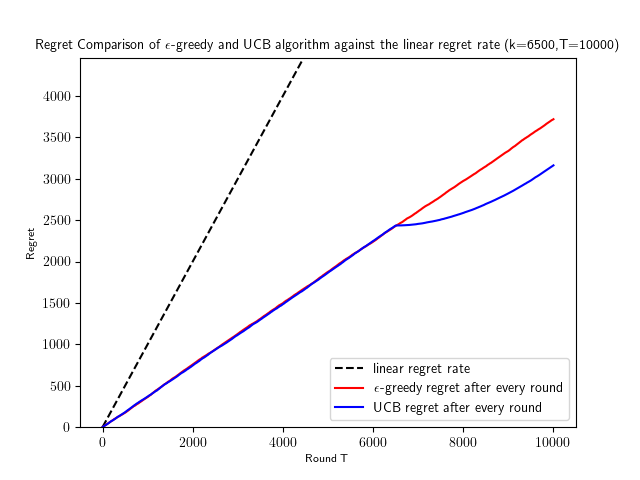
\includegraphics[width=\textwidth]{fig8.png}
					\caption{$(k=6500, T=10000)$}
				\end{subfigure}
				\hfill
				\begin{subfigure}[b]{0.3\textwidth}
					\centering
					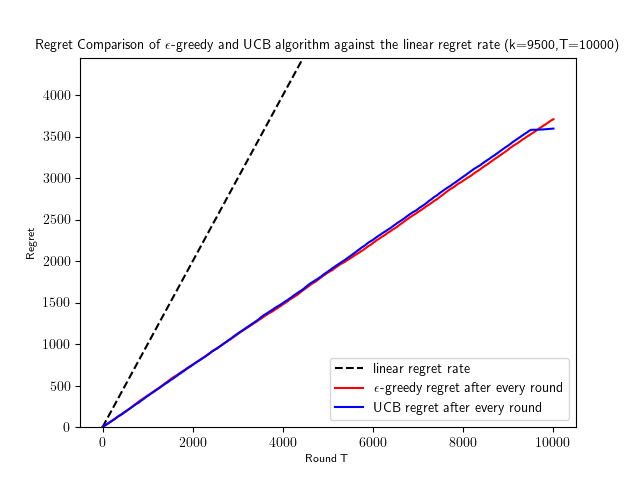
\includegraphics[width=\textwidth]{fig10.png}
					\caption{$(k=9500, T=10000)$}
				\end{subfigure}
				\caption{$(k\in[100,9500], T=10000)$}			
			\end{figure}
		
			The experiments of figure 1 where tested again for different values of $k,T$ but with the same $\frac{k}{T}$ ratios. As shown in figure 2 the algorithms present the same behaviors observed in figure 1.
		\end{enumerate}
	
\end{document}
